\chapter{Algoritmos de Ordenação}

O problema da ordenação é central na análise de algoritmos por dois motivos.
Em primeiro lugar, ele é um problema com muitas aplicações em diversas áreas da computação.
Em segundo lugar, são conhecidas diversas soluções bem diferentes para esse problema, o que o torna um excelente exemplo para a teoria que estamos apresentando.

Vamos relembrar o problema:

  {\bf Problema da ordenação}\\

  {\bf Entrada:} Uma sequência de $n$ valores $a_1, \dots, a_n$ em que $a_i \in \mathbb{Z}$ para $1 \leq i \leq n$.\\

  {\bf Saída:} Uma permutação da sequência de entrada $a'_1, \dots, a'_n$ tal que $a_i \leq a_j$ para todo $i < j$.

  \section{Selection Sort}

  Comecemos com uma solução bem simples para o problema, um algoritmo chamado Selection Sort.
  Esse algortimo consiste em identificar o maior elemento da sequência e trocá-lo com o último e repetir o processo até que todos estejam em ordem.

  Assim, podemos começar com a seguinte sub-rotina:

  \begin{codebox}
\Procname{$\proc{Maximo}(A)$}
\li \Comment Recebe uma sequência $a_1, \dots, a_n$
\li \Comment Devolve $i$ tal que $a_i$ é o maior elemento da sequência
\li $imax \gets 0$
\li \For $i \gets 2$ até $n$
\li \Do \If $a_i > a_{imax}$
\li     \Then $imax \gets i$
        \End
    \End
\li \Return $imax$
\End
  \end{codebox}

  Para provar que este algoritmo é correto, note que a seguinte propriedade é invariante na linha 2:

  \begin{center}
    $a_{imax}$ é o maior elemento em $a_i, \dots, a_{i-1}$ 
  \end{center}

  {\em Inicialização:} na primeira vez que passamos pela linha 2 temos que $i = 2$.
  Portanto, a sequência $a_1, \dots, a_{i-1}$ tem apenas um elemento ($a_1$) que só pode ser o maior.

  {\em Manutenção:} se na iteração anterior $a_{imax}$ era o maior elemento em $a_1, \dots, a_{i-1}$ temos duas possibilidades: se $a_i$ fosse maior que $a_{imax}$ então teríamos atualizado $imax$ e ele continuaria sendo o maior da sequência, caso contrário $imax$ não teria sido atualizado, mas $a_{imax}$ continuaria sendo o maior elemento.

  {\em Término:} quando chegamos na linha 5 temos que $a_{imax}$ é o maior elemento de $a_1, \dots, a_n$.

  Analisar o tempo de processamento deste algoritmo também é simples.
  Para facilitar as contas, faremos mais uma simplificação.
  Ao invés de somar o tempo de processamento de cada linha, calcularemos o tempo apenas de uma das linhas que mais se repete, neste caso escolhemos a 3.
  Essa linha é processada $n$ vezes e, portanto, o algortimo é $\Theta(n)$.

  Apresentemos agora o algoritmo Selection Sort.

  
  \begin{codebox}
\Procname{$\proc{SelectionSort}(A)$}
\li \For $j \gets n$ até $2$
\li \Do $imax \gets Maximo(a[1:j])$
\li     \Then $a_{imax} \leftrightarrow a_j$
        \End
    \End
\End
  \end{codebox}

  A propriedade invariante na linha 2, neste caso, é:
  \begin{center}
    a sequência $a_j, \dots, a_n$ está em ordem crescente
  \end{center}

  {\em Inicialização:} na primeira passagem temos que $j=n$ e, portanto a squência $a_j, \dots, a_n$ tem um único elemento $a_n$.

  {\em Manutenção:} pela hipótese de indução $a_j, \dots, a_n$ estava ordenada na iteração anterior, assim basta mostrar que $a_{j-1} < a_j$, mas isso é o caso porque o algoritmo garante que $a_j$ é o maior elemento de $a_1, \dots a_j$.
  

  Para analisar o tempo de processamento deste algoritmo, consideraremos a linha 2 que se repete $n$ vezes.
  A operação executada nessa linha, porém, não é atômica.
  Como vimos, ela toma tempo proporcional ao tamanho da entrada que varia em cada iteração.
  Na primeira iteração toma tempo proporcional a $n$, na segunda $n-1$, então $n-2$ e assim por diante.

  O tempo de processamento em função do tamanho $n$ da entrada, então, é:

  \begin{displaymath}
    T(n) = n + (n-1) + (n-2) + \dots + 1 = \sum_{i=1}^{n}i = \frac{n(n+1)}{2} \in \Theta(n^2)
  \end{displaymath}

  Assim se calcularmos o tempo de processamento de uma implementação desse algoritmo para entradas de diferentes tamanhos, devemos observar uma parábola (Figura \ref{}):

  \begin{figure}
    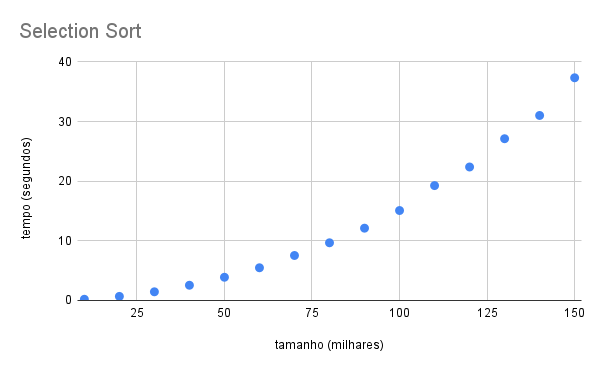
\includegraphics[width=\textwidth]{imagens/SelectionSort1.png}
  \end{figure}

  Podemos testar que se trata de fato de uma parábola poltando os mesmo valores em um gráfico em que ambos os eixos estão em escala logarítmica.
  Se a função tiver o formato $T(n) = an^2$, como nossa análise sugere, ao aplicar o $log$ nos dois lados, temos que:
  \begin{displaymath}
  log(T(n)) = log(an^2) = 2log(n) + log(a)
  \end{displaymath}
  
  Assim, o que obtemos é a equação de uma reta com inclinação $2$.
  Na Figura \ref{} observamos que de fato em uma gráfico log-log o que obtemos é uma reta com inclinação $1,94$, valor bem próximo do esperado.

  \begin{figure}
    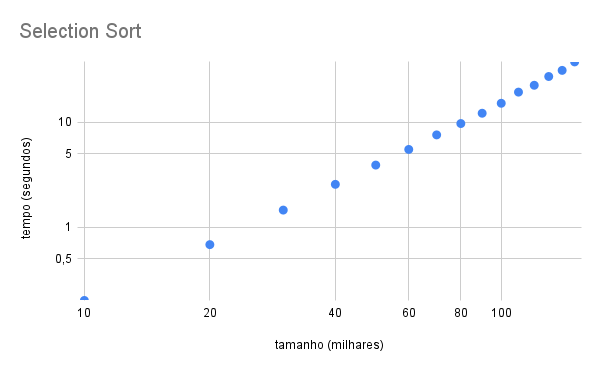
\includegraphics[width=\textwidth]{imagens/SelectionSort2.png}
  \end{figure}

  
\section{Insertion Sort}
\section{Merge Sort}
\section{Quick Sort}
\section{Heap Sort}
